\documentclass[a4paper,12pt]{article}

\usepackage[utf8]{inputenc}
\usepackage[T1]{fontenc}
\usepackage[brazil]{babel}
\usepackage{graphicx}
\usepackage{xcolor}
\usepackage{tcolorbox}
\usepackage{geometry}
\usepackage{tikz}
\usetikzlibrary{positioning, shapes.multipart}
\geometry{margin=2.5cm}
 
\definecolor{meuazul}{RGB}{0, 79, 151}

\begin{document}

\begin{center}
    
\includegraphics[width=3cm]{logo.png} \\
    \vspace{0.5cm}
    \textbf{\large Engenharia da Qualidade e Confiabilidade} \\
    \textbf{Atividade Prática: Planning Poker}
\end{center}

\vspace{1cm}

\begin{tcolorbox}[colback=meuazul!5, colframe=meuazul, title=\textbf{HU001: Gerenciamento de Rebanho Leiteiro}]
    
    \textbf{Título:} Gestão Completa de Vacas para Ordenha
    
    \vspace{0.3cm}
    \textbf{Descrição (História de Usuário):} \\
    Como \textbf{Encarregado da Ordenha}, \\
    quero \textbf{cadastrar, visualizar, atualizar e remover vacas do rebanho}, \\
    para \textbf{garantir o controle individual da produção leiteira, rastreabilidade e acompanhamento da saúde dos animais}.
    
    \vspace{0.3cm}
    \textbf{Valor de Negócio:} \\
    Permite melhor tomada de decisão, controle sanitário e aumento da produtividade.
    
    \vspace{0.3cm}
    \textbf{Prioridade:} Alta
    
\end{tcolorbox}

\vspace{0.5cm}

\section*{Story Points e Protótipos de Tela}
\begin{enumerate}
    \item \textbf{Cadastrar Vaca:} Inserir Brinco (único), Nome, Raça, Data de Nascimento e Status inicial.
    \begin{itemize}
        \item \textit{Explicação:} A tela de cadastro permite ao operador registrar um novo animal no sistema, validando o identificador (brinco) para evitar duplicidade.
        \begin{center} 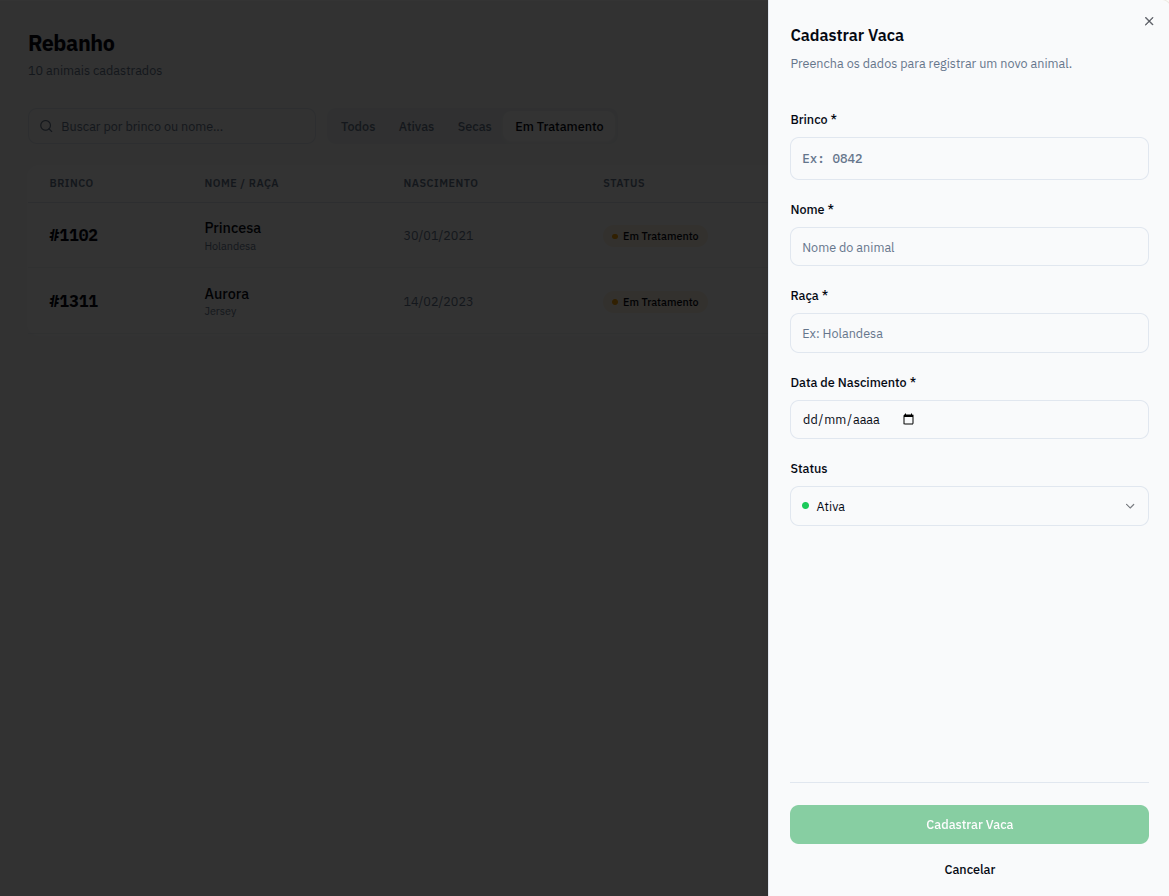
\includegraphics[width=\textwidth]{criar.png} \end{center}
    \end{itemize}

    \item \textbf{Visualizar Lista:} Listagem com filtros por status (Ativa, Seca, Tratamento) e busca por brinco.
    \begin{itemize}
        \item \textit{Explicação:} Exibe o rebanho completo, permitindo buscas rápidas e filtragem para identificar quais animais estão em produção ou em tratamento sanitário.
        \begin{center} 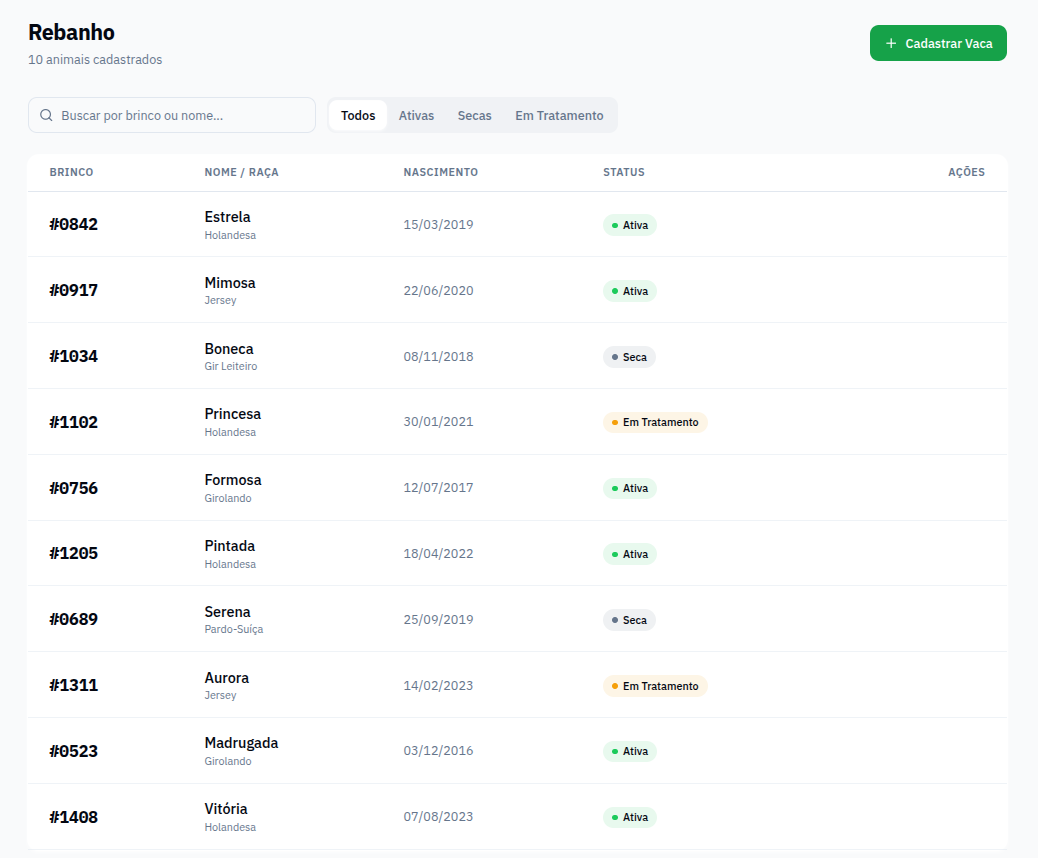
\includegraphics[width=\textwidth]{exibir.png} \end{center}
    \end{itemize}

    \item \textbf{Atualizar Dados:} Permitir edição de todos os campos e alteração de status.
    \begin{itemize}
        \item \textit{Explicação:} Utilizada para manter os dados atualizados, como mudanças de fase (ex: de Ativa para Seca) ou correção de informações cadastrais.
        \begin{center} 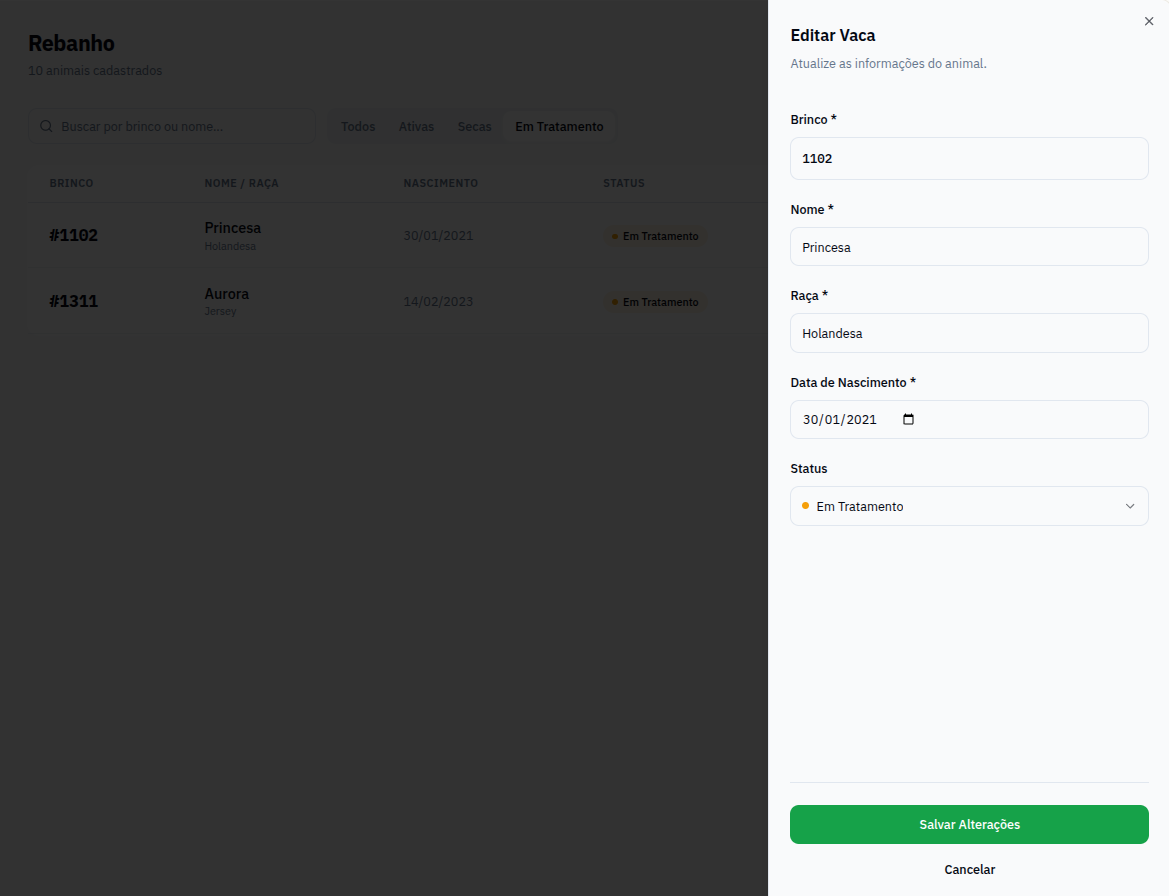
\includegraphics[width=\textwidth]{editar.png} \end{center}
    \end{itemize}

    \item \textbf{Excluir Registro:} Remoção permitida apenas se não houver registros de ordenha vinculados.
    \begin{itemize}
        \item \textit{Explicação:} Garante a integridade dos dados, impedindo que um animal com histórico de produção seja removido acidentalmente.
        \begin{center} 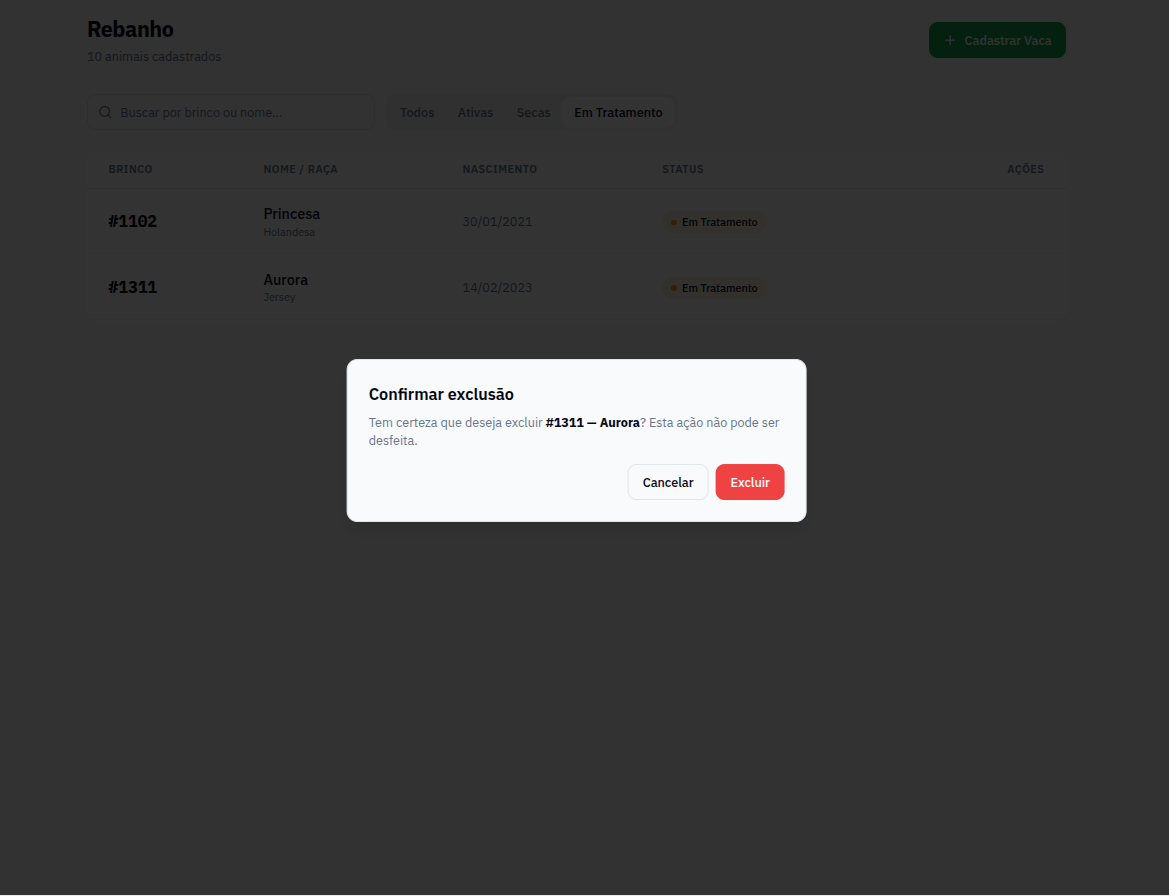
\includegraphics[width=\textwidth]{excluir.png} \end{center}
    \end{itemize}
\end{enumerate}

\vspace{0.5cm}

\section*{Modelo de Dados (Diagrama de Classes)}

Para auxiliar na estimativa, considere o seguinte modelo simplificado das entidades envolvidas:

\begin{center}
\begin{tikzpicture}[
    node distance=2cm,
    classBox/.style={
        draw=meuazul,
        thick,
        fill=white,
        minimum width=4cm,
        rectangle split,
        rectangle split parts=3,
        align=left,
        rounded corners=2pt
    }
]

% Classe Vaca
\node[classBox] (Vaca) {
    \textbf{Vaca}
    \nodepart{second}
    - brinco: String \{PK\} \\
    - nome: String \\
    - raca: String \\
    - dataNascimento: Date \\
    - status: StatusVaca
    \nodepart{third}
    + validarBrinco() \\
    + calcularIdade()
};

% Classe Ordenha
\node[classBox, right=3cm of Vaca] (Ordenha) {
    \textbf{Ordenha}
    \nodepart{second}
    - id: Integer \{PK\} \\
    - data: DateTime \\
    - litros: Float \\
    - observacao: Text
    \nodepart{third}
    + registrarProducao()
};

% Associação
\draw[thick, meuazul] (Vaca) -- (Ordenha) 
    node[pos=0, above right] {1} 
    node[pos=1, above left] {*};

\end{tikzpicture}
\end{center}

\vspace{0.5cm}

\section*{Atividade: Estimativa com Planning Poker}

Cada grupo deverá estimar o esforço das funcionalidades utilizando \textbf{Story Points} com base na sequência de Fibonacci:

\begin{center}
\textbf{0, 1, 2, 3, 5, 8, 13, 21}
\end{center}

\vspace{0.3cm}

\textbf{Instruções:}
\begin{enumerate}
    \item O professor (PO) apresenta a História de Usuário.
    \item A equipe discute dúvidas e entende os requisitos.
    \item Cada aluno escolhe uma carta (sem mostrar aos demais).
    \item Todos revelam simultaneamente.
    \item Em caso de divergência, discutir e votar novamente até consenso.
\end{enumerate}

\vspace{0.5cm}

\section*{Registro das Estimativas}


\vspace{1cm}

\begin{center}
    \rule{0.5\textwidth}{0.4pt} \\
    \small UniRV - Engenharia de Software
\end{center}

\end{document}